\listoftodos



\chapter{Grundlagen}
\label{chap:Grundlagen}

	\section{TODO GRUNDALGENDETAIL}
	\label{sec:TODOGrundlagenDetail}
		\todo{notwendige klassische Grundlagen definieren} 
	\section{Bestehendes System}
	\label{sec:BestehendesSystem}
			(Object Detection - AutoCrane)

	\section{Datenverständnis}
	\label{sec:DataUnderstanding}
	Anlehnend dem in Kapitel \ref{sec:Vorgehen} beschriebenen Vorgehen \todo{Vorgehen auch so beschreiben /  ansonsten Kapitel Einleitung anpassen} werden in diesem Kapitel die zur Verfügung stehenden Daten und deren Qualität beschrieben. Dabei ist das Kapitel entsprechend der Beschriftung der Daten in zwei Teilbereiche unterteilt.
	
	Im Rahmen des bestehenden Autocrane-Projektes \ref{sec:BestehendesSystem} \todo{Im Kapitel Bestehdens System erwähnen / diesen Teil in das andere Kapitel verschieben?} wurde eine Kamera an einem Kran angebracht. Die Kamera ist so ausgerichtet, dass sich Aufhängung des Greifers am mittleren oberen Bildrand befindet. Die Auslenkung kann jeden Winkel in einem 360 Grad Radius um das Zentrum des Krans erreichen. Der Hintergrund der Bilder kann sich somit stark ändern. Mittels der Kamera werden kontinuirlich neue unbeschriftete Bilder aufgenommen und bei PSIORI abgelegt. Zu Beginn dieser Arbeit standen mehr 385.000 nicht beschriftete Bilder zur Verfügung. Die Bilder sind 1024 auf 648 Pixel groß und in Farbe. Sie sind in der Form (1024, 648, 3). Die einzelnen Pixel können dabei Werte zwischen 0 und 255 annehmen. 
	Zum Erreichen der Zielstellung werden zwei Datensätze benötigt.
	
		\paragraph{Greifer Datensatz} Der Greifer Datensatz enthält Bilder, in welchen der Greifer mittels Rahmen markiert ist. Abbildung \ref{img:Logs}  zeigt ein beispielhaftes Bild mit markiertem Greifer. Abbildung \ref{img:Grapple} zeigt ein beispielhaftes Bild mit markiertem Greifer.
		\begin{figure}[h]
				\centering
				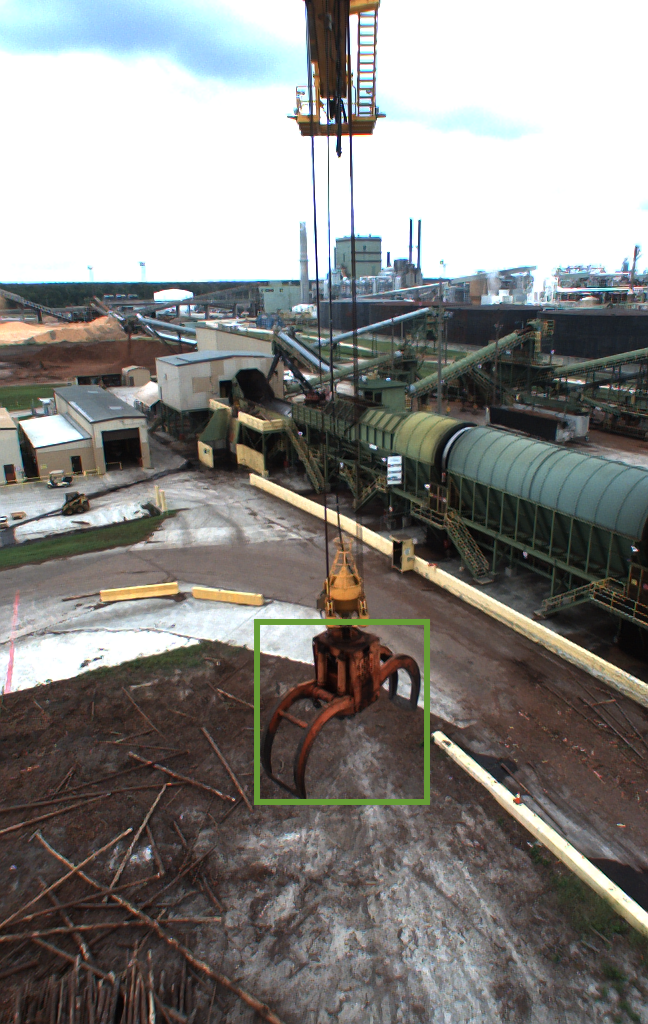
\includegraphics[width=0.5\textwidth, center]{bilder/Grundlagen/Grapple_8.png}
				\caption[Bsp. Bild: Greifer mit Rahmen]{Greifer mit Rahmen}
				\label{img:Grapple}
		\end{figure}
		Der Datensatz besteht aus zwei Sammlungen von qualitativ unterschiedlich gut beschrifteten Bildern. Die eine Sammlung besteht aus einem bestehenden Datensatz, welcher 4.684 durch Menschen annotierten Bildern enthält. Für den zweiten Teil der Sammlung wurden mittels der \todo{siehe Bestehendes System} bestehenden Objekterkennung XXXX Bilder annotiert. \todo{Vorgehen + Metriken detailierter beschreiben} Das genaue Schema der Datenstrukturen kann in Anhang \ref{appendix:AutocraneDaten} nachgelesen werden.

		\paragraph{Baumstamm Datensatz} Der Baumstamm Datensatz enthält Bilder, welche die Annotation, ob sich Baumstämme im Greifer befinden haben. Abbildung \ref{img:Logs} zeigt ein Bild, in welchem der Greifer Baumstämme greift. In Abbildung \ref{img:Grapple} befinden sich keine Baumstämme im Greifer.
		\begin{figure}[h]
			\centering
			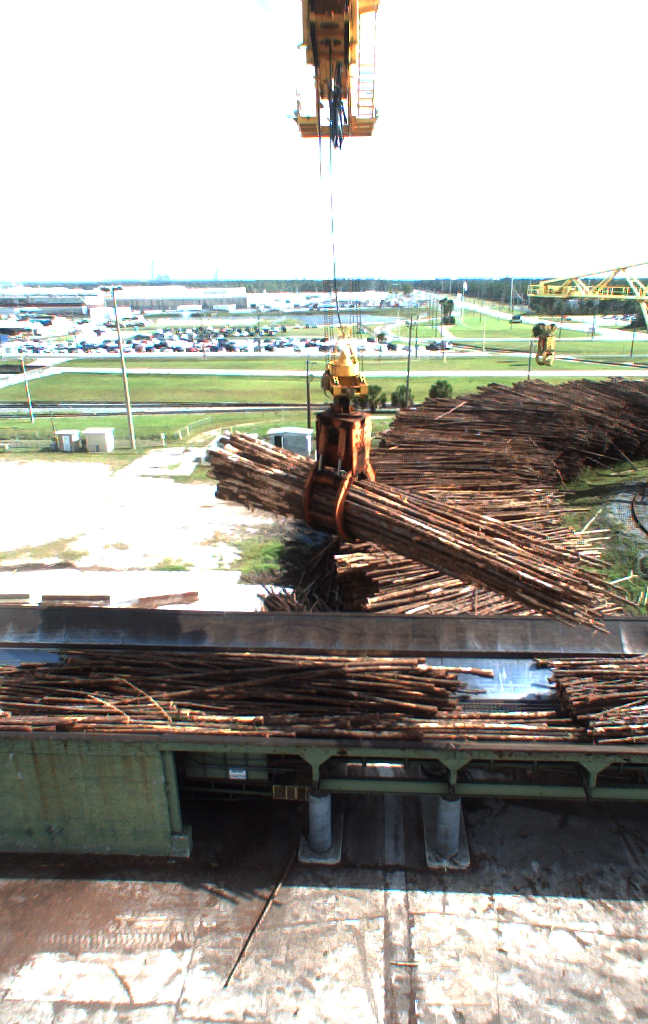
\includegraphics[width=0.5\textwidth, center]{bilder/Grundlagen/Logs_14.png}
			\caption[Bsp. Bild: Greifer mit Baumstämmen]{Greifer mit Baumstämmen}
			\label{img:Logs}
		\end{figure}
		Der Datensatz wurde mittels Crowd
			
	%		\begin{figure}[h]
	%		\centering
	%		\includegraphics[width=0.5\textwidth, center]{bilder/Grundlagen/.png}
	%		\caption[Bsp. Bild: Greifer mit Baumstämmen]{Greifer mit Baumstämmen}
	%		\label{img:Helligkeit}
	%		\end{figure}			
		

				
		 \todo{Brightness-Histogramm einfügen} 
			
				 Im Rahmen des Datenverständnisses wird versucht, sich einen ersten Überblick über die zur Verfügung stehenden Daten und deren Qualität zu verschaffen. Es erfolgt eine Analyse und Bewertung der Datenqualität. Probleme mit der Qualität der vorhandenen Daten in Bezug auf die in der vorherigen Phase festgelegten Aufgabenstellung sind zu benennen.
			
			todo? Datenqualität auf helle und dunkle bidler verweisen und somit zu Datenvorbereitung: skalierung 0-1 verweissen
		
	\section{Datenvorbereitung}
	\label{sec:DataPreparation}

Die Datenvorbereitung dient dazu, einen finalen Datensatz zu erstellen, der die Basis für die nächste Phase der Modellierung bildet.


			In dem Schritt Datenvorbereitung werden die Bilder für die Modellerstelung vorbereitet. In dieser Arbeit wurde für diesen Schritt eine Klasse Preprocessing in einem neuen Modul data\_preperation.py  erstellt. Wie in Listing 
			% \lstinputlisting[language=Python,caption={Preprocessing},label=lst:Preprocessing]{\srcloc/data\_preperation.py }
			
			 zu sehen werden die Pixel der Bilder zwischen 0 und 1 Skaliert. Dei Skalierung erfolgt damit jedes Bild eine ähnliche Gewichtung
			
			Neural networks process inputs using small weight values, and inputs with large integer values can disrupt or slow down the learning process. As such it is good practice to normalize the pixel values so that each pixel value has a value between 0 and 1.
	Die Bilddaten werden 		


	\begin{table}[ht]
	\centering
	\begin{tabularx}{\textwidth}{lllll}
		 & \textbf{Train} & \textbf{Test}  & \textbf{Validation} & \textbf{Summe} 								  \\
		\textbf{Greifer} 				 & 	X					&	X					& 4.684 				   & x 				\\
		\textbf{Baumstämme T/F}	 	  &  X					 &	X					 &	X							& 18000		\\
	\end{tabularx}

	\caption{Datenaufteilung - Train Test Validation}
	\label{table:DatenaufteilungTrainTestValidation}
 	\end{table}
 
	\section{Bibliotheken und Werkzeuge}
	\label{sec:BibliothekenundWerkzeuge}
		\paragraph{Tensorflow}
		\paragraph{Keras}
		\paragraph{Psipy} ist ein Python-Framework für Maschinelles Lernen welches von PSIORI selbst entwickelte Modelle zusammenfasst und eine einheitliche API zu Verfügung stellt. Diese API ist an die API des verbreiteten Frameworks scikit-learn angelehnt und die Modelle aus scikit-learn können in das von PSIORI entwickelte Framework eingebunden werden. Das Framework ermöglicht außerdem das Einbinden von Modellen basierend auf TensorFlow.\grqq [PSIORI]
		\paragraph{Cnvrg.io} \todo{Quelle cnvrg} ist eine "full-stack Data Science Platform" welche Werkzeuge  für die Erstellung, Verwaltung, Bereitstellung  und Automatisierung von maschinellem Lernen bereitstellt. \todo{mehr Text; was wurde genutzt (Datasets,...)}
			
	\section{Experimentumgebung}
	\label{sec:Experimentumgebung}
		(Hardware + eingesetzte Software)